\documentclass[tikz,border=2pt]{standalone}
\usepackage{amsmath}
\usepackage{pgfplots}
\pgfplotsset{compat=1.18}
\usetikzlibrary{arrows.meta}
\begin{document}
% f(x) = sin(3x) has fundamental period T = 2*pi/3: the graph on one window [0, T] (shaded)
% is repeated by shifts of T; the points x and x + T have the same height.
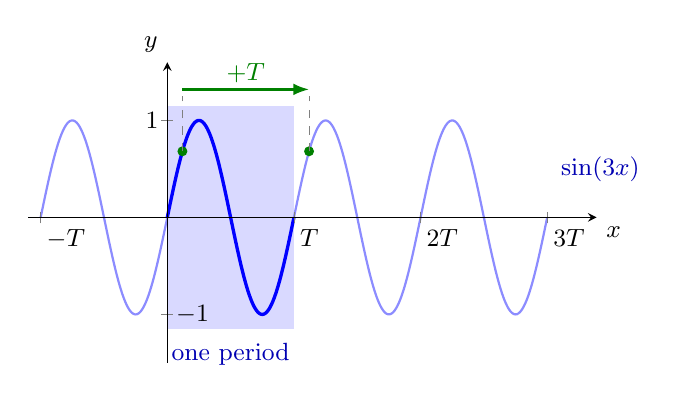
\begin{tikzpicture}[font=\small, >={Latex[length=2mm]}]
  \begin{axis}[
    axis lines=middle,
    xmin=-2.3, xmax=7.1, ymin=-1.5, ymax=1.6,
    xtick={-2.0944,2.0944,4.1888,6.2832},
    xticklabels={$-T$,$T$,$2T$,$3T$},
    ytick={-1,1}, yticklabels={},
    xticklabel style={anchor=north west, inner sep=2pt},
    xlabel={$x$}, ylabel={$y$},
    xlabel style={below right}, ylabel style={above left},
    samples=160, smooth, clip=false,
    width=8.8cm, height=5.4cm, axis on top
    ]
    \fill[blue!15] (axis cs:0,-1.15) rectangle (axis cs:2.0944,1.15);
    \addplot[blue!45, thick, domain=-2.0944:0] {sin(deg(3*x))};
    \addplot[blue, very thick, domain=0:2.0944] {sin(deg(3*x))};
    \addplot[blue!45, thick, domain=2.0944:6.2832] {sin(deg(3*x))};
    \node[blue!70!black, anchor=west] at (axis cs:6.35,0.5) {$\sin(3x)$};
    \node[anchor=east, inner sep=3pt] at (axis cs:0,1) {$1$};
    \node[anchor=west, inner sep=3pt] at (axis cs:0,-1) {$-1$};
    % f(x) = f(x+T)
    \fill[green!50!black] (axis cs:0.25,{sin(deg(0.75))}) circle (1.8pt);
    \fill[green!50!black] (axis cs:2.3444,{sin(deg(0.75))}) circle (1.8pt);
    \draw[->, green!50!black, thick] (axis cs:0.25,1.32) -- node[above, inner sep=2pt] {$+T$} (axis cs:2.3444,1.32);
    \draw[gray, thin, dashed] (axis cs:0.25,{sin(deg(0.75))}) -- (axis cs:0.25,1.25);
    \draw[gray, thin, dashed] (axis cs:2.3444,{sin(deg(0.75))}) -- (axis cs:2.3444,1.25);
    \node[blue!70!black, anchor=north] at (axis cs:1.0472,-1.2) {one period};
  \end{axis}
\end{tikzpicture}
\end{document}
